%
% File eacl2009.tex
%
% Contact  oflazer@gmail.com or das@ling.uni-potsdam.de
%%

%% Based on the style files for EACL 2006 by 
%%e.agirre@ehu.es or Sergi.Balari@uab.es
%% and that of ACL 08 by Joakim Nivre and Noah Smith

\documentclass[11pt]{article}
\usepackage{eacl2009}
\usepackage{times}
\usepackage{url}
\usepackage{latexsym}
\usepackage[icelandic]{babel}
\usepackage[T1]{fontenc}
\usepackage[utf8]{inputenc}
\usepackage{graphicx}
\usepackage{wrapfig}

\setlength\titlebox{9.5cm}    % You can expand the title box if you
% really have to

\title{Rýnir - Tækniskýrsla}

\author{Arnór Barkarson\\
  Reykjavík University\\
  Reykjavík, Iceland\\
  {\tt arnorbarkar@ru.is}  \And  
  Ragnar Lárus Sigurðsson\\
  Reykjavík University\\
  Reykjavík, Iceland\\
  {\tt  ragnarls08@ru.is}\\ \And 
  Þórður Arnarsson\\
  Reykjavík University\\
  Reykjavík, Iceland\\
  {\tt  thordura08@ru.is}  \And 
  Gunnar Sveinsson\\
  Reykjavík University\\
  Reykjavík, Iceland\\
  {\tt  gunnarsve06@ru.is} 
}



\date{}

\begin{document}
\maketitle

\section{Aðferðir notaðar í Rýni}
\subsection{Fourier transformations}
Fourier transformations eru stærðfræðilegar aðgerðir sem brjóta merki niður í tíðnir þess. Slíkt gátum við nýtt okkur með því að láta umbreyta 
tímalínu í tíðnir. Ef áberandi tíðni fannst þá er endurtekning í tímalínunni. Sem dæmi um slíkt er þegar 
rafmagnsnotkun í ótilgreindu landi er skoðuð.\\
\begin{wrapfigure}{l}{6cm}
%\begin{figure}
 \begin{center}
 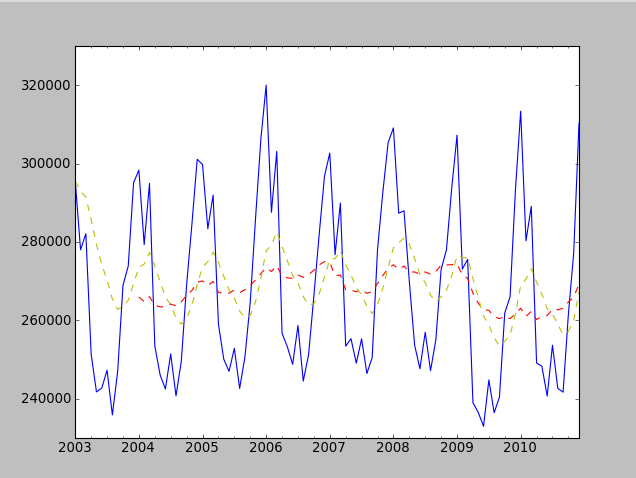
\includegraphics[width=.45\textwidth]{Rafmagnsnotkun.png}
 \caption{Tímalína um rafmagnsnotkun}
  \end{center}
%\end{figure}
\end{wrapfigure}
\hfill
\\\\\\\\\\\\\\\\\\\\\\\\\\\\\\\

Það má sjá að tímalínan hefur ákveðnar endurtekningar, nánar til tekið þá er mikil notkun á veturna en lítil á sumrin.
Þessa föstu sveiflu í tímalínunni greinir Fourier og skilar eftirfarandi grafi. 
Það segir okkur að á 12 staka fresti í tímalínunni er endurtekning.
\begin{wrapfigure}{l}{6cm}
%\begin{figure}
 \begin{center}
 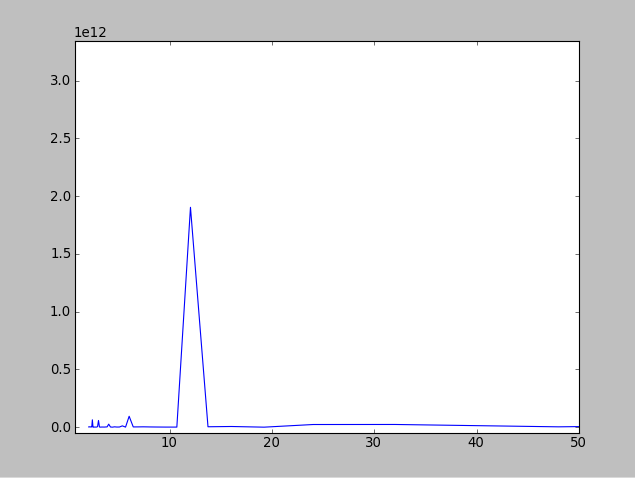
\includegraphics[width=.45\textwidth]{Fourier.png}
 \caption{Fourier um rafmagnsnotkun}
  \end{center}
%\end{figure}
\end{wrapfigure}
\hfill
\\\\\\\\\\\\\\\\\\\\\\\\\\\\\\\

\subsection{Hlaupandi meðaltal (HM)}
Í tölfræði er hlaupandi meðaltal, einnig kallað fljótandi meðaltal, notað til greiningar á gagnamengi. 
Er það gert með því að mynda röð meðaltala úr mismunandi hlutmengjum heildarmengisins.\\
Ef gefin er röð $Z$ talna og ákveðin stærð ramma (hlutmengis) er $N$, þá er fljótandi meðaltal fundið með því að fyrst reikna meðaltal 
talna úr sæti $0,1,\dots,N-1$. Þá er ramminn færður fram um eitt sæti og meðaltal fundið af tölum í sætum $1,2,\dots,N$. 
Þessi aðgerðarröð er endurtekin yfir alla talnaröðina, $Z-N$ sinnum.  \\
$HM = \frac{x+(x+1)+\dots+(x+(N-1))}{N}$
\\
Línan sem tengir svo saman öll meðaltölin er hið fljótandi meðaltal þar sem hver punktur á línunni samsvarar 
meðaltali viðkomandi hlutmengis í heildarmengi ganganna sem verið er að meta. 
 
\subsection{Vegið hlaupandi meðaltal (VHM)}
Hlaupandi meðaltal getur einnig notað ójöfn gildi fyrir hvert stak á línunni.
Þá er um vegið meðaltal að ræða og er meðaltalinu gefin einhver margfeldisáhrif eftir því hvar á línunni það er staðsett. 
Það vægi breytist línulega. Summu margfeldi allra gildana í tilteknum ramma er svo deilt með summu allra mergfeldanna. 
Ef um ramma af stærð 10 er að ræða og gildin eru margfölduð eftir sætisröð, þá fæst: \\
$VHM = \frac{x+2(x+1)+3(x+2)+\dots+(10(N-1))}{1+2+\dots+10}$
\subsection{Bollinger bands}
\label{sec:third}
Bollinger bönd eru upprunalega þróuð sem greiningartól á þróun verðbréfaverða. 
Tilgangur þeirra er að veita viðeigandi skilgreiningu háum og lágum gildum. Einnig hefur þessari aðferð verið beitt á ýmis önnur
vandamál með misgóðum niðurstöðum. \\
Bollinger bönd samanstanda af
\begin{itemize}
  \item Miðband, $N-lotu$ einfalt hlaupandi meðaltal.
  \item Efra band, $N-lotu$ staðalfrávik margfaldað með $K$, fyrir ofan miðbandið ($HM + K\sigma$).
  \item Neðra band, $N-lotu$ staðalfrávik margfaldað með $K$, fyrir neðan miðbandið ($HM - K\sigma$).%\\\\\\\\\\\\\\\\\
\end{itemize}

\begin{wrapfigure}{l}{6cm}
%\begin{figure}
 \begin{center}
 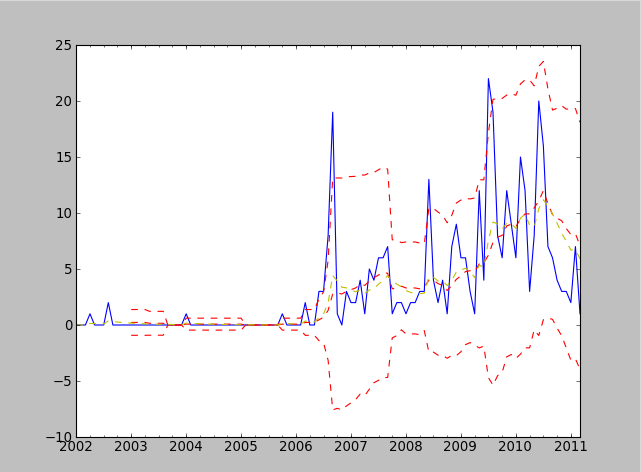
\includegraphics[width=.45\textwidth]{Bollinger.png}
 \caption{Rauðu strikalínurnar sýna Bollinger böndin}
  \end{center}
%\end{figure}
\end{wrapfigure}
\hfill
\\\\\\\\\\\\\\\\\\\\\\\\\\\\\\\\\\
Bollinger bönd nýtast því vel til greininga hvar í tímalínu óeðlileg hækkun eða lækkun á sér stað.
\\
\subsubsection{Okkar útfærsla á Bollinger}
Útfærslan okkar byggist á því að ítra í gegnum mismunandi stórar rammastærðir fyrir hverja tímalínu.
Hver rammastærð gefur hverjum punkti einkunn út frá því hvar punkturinn er staddur með tilliti til Bollinger bandanna.
Til þess ákváðum við að nota breytta útgáfu af því sem kallast $\%b$ sem gefur punkti gildi yfir 1 ef punkturinn er fyrir utan 
efri mörk Bollinger bandsins, tölugildi á bilinu 1-0 ef punkturinn liggur á milli þeirra og neikvæða tölu ef hann er undir þeim.
$\%b={(last-lowerBB)}{(upperBB-lowerBB)}$
Við notum breytta útgáfu af formúlunni sem hundsar hvort við erum fyrir ofan eða neðan böndin og gefur einfaldlega gildi á bilinu
0-1 ef punkturinn liggur á milli bandanna en annars gildi yfir einum ef punkturinn er fyrir utan. Haldið er utan um hvort punkturinn 
lá fyrir ofan eða neðan í flagginu sjálfu.
$\%b=\frac{abs((item - avg[index])}{(upperlim[index] - avg[index]))}$
Hver rammastærð margfaldar sína útkomu úr formúlunni við gildið sem punkturinn hefur fyrir.
Þannig gefum við punktum sem líta út fyrir að vera snörp hækkun í litlum ramma lækkað vægi þegar hann lendir innan bandanna í stærri ramma
og telst því til eðlilegrar hegðunar þegar horft er lengra aftur í tímann.
Punktar sem leggja utan Bollinger bandanna í nokkrum rammastærðum fá einnig aukið vægi þar sem hver rammi hækkar gildið.

Ef að í tímalínunni er tímabil sem inniheldur svipaðar eða eins tölur á kafla sem er stærri en rammastærðin er vandamál að Bollinger 
böndin þrengjast mikið. Það gerði það að verkum að litlar breytingar eftir þannig tímabil voru gefin óeðlilega hátt gildi, 
jafnvel töluvert hærra gildi en það sem teldist til mikið áhugaverðari punkta í sjón. Til að koma í veg fyrir þetta er notast við
einfalda athugun sem skoðar hvort bandbreiddin fyrir viðkomandi punkt er óeðlilega þröng miðað við meðalbandbreidd tímalínunnar.
Ef svo er er punktinum gefið lægra gildi. Þegar þetta er skrifað er notast við fasta margföldun en hugmyndir eru uppi um að lækka 
gildið útfrá meðaltali gilda í tímalínunni.

Að lokum hreinsum við flögg sem liggja hlið við hlið, liggja sömu megin Bollinger bandanna og innihalda sífellt hækkandi gildi, 
þannig skilum við einungis toppum á hækkunum sem kerfið sér, en ekki punkta innan hækkunaninnar.

 



\end{document}
